\documentclass[xcolor={svgnames},12pt,aspectratio=169,handout]{beamer}
\usetheme{Berlin}
\usecolortheme{dolphin}

\setbeamercolor*{structure}{bg=Azure,fg=MidnightBlue!50!black}

\setbeamercolor*{palette primary}{use=structure,fg=structure.bg,bg=structure.fg}
\setbeamercolor*{palette secondary}{use=structure,fg=structure.fg,bg=structure.bg}
\setbeamercolor*{palette tertiary}{use=structure,fg=structure.fg,bg=GhostWhite}
\setbeamercolor*{palette quaternary}{fg=white,bg=black}

\setbeamercolor{section in head/foot}{parent=palette primary} % Outer section of header/footer
\setbeamercolor{subsection in head/foot}{parent=palette secondary} % Inner section of header/footer

\setbeamercolor{titlelike}{parent=palette tertiary} % Main titles
\setbeamercolor{frametitle}{parent=palette tertiary,bg=GhostWhite!50}

\setbeamercolor{section in toc}{fg=darkgray,bg=Azure} % Table of contents sections
\setbeamercolor{subsection in toc}{fg=darkgray,bg=Azure} % Table of contents subsections
% \setbeamercolor{alerted text}{use=structure,fg=structure.fg!50!black!80!black}

% \setbeamertemplate{navigation symbols}{} % Hides navigation buttons at the bottom
% \setbeamertemplate{headline}{} % Hides navigation bar at the top
\setbeamercovered{transparent}

% \usepackage{pgfpages}
% \pgfpagesuselayout{4 on 1}[a4paper,border shrink=5mm]

\usepackage[utf8]{inputenc}
\usepackage[all]{xy}
\usepackage{tikz}
\usetikzlibrary{mindmap,backgrounds}
\usepackage{graphicx}
\usepackage{multicol}
% Advanced table functions
\usepackage{tabularx,ragged2e}
\usepackage{booktabs}
% Listings extension
\usepackage{listings}

\title[Empowering Users' Privacy Rights in the Internet of Things]{Master's Thesis Preparation \\ {\normalsize Empowering Users' Privacy Rights in the Internet of Things}}
% \subtitle{Empowering Users' Privacy Rights in the Internet of Things}
\author{\href{mailto:2080511@student.uma.pt}{Nelson Vieira}}
\institute[\href{https://www.uma.pt/}{University of Madeira}]{University of Madeira\\Faculty of Exact Sciences and Engineering}
\date{Last Update: \today}

\setbeameroption{show notes}

\makeatletter
    \newenvironment{withoutheadline}{
        \setbeamertemplate{headline}[default]
        \def\beamer@entrycode{\vspace*{-\headheight}}
    }{}
\makeatother

\begin{document}

\begin{withoutheadline}
    \begin{frame}
        \centering
\includegraphics[width=100pt]{../assets/images/uma_logo.png}
        \maketitle
    \end{frame}
\end{withoutheadline}

\begin{frame}{Table of Contents}
    % Use hideallsubsections for longer presentations
    % \tableofcontents[hideallsubsections]
    \begin{multicols}{2}
        \tableofcontents
    \end{multicols}
\end{frame}

\section{Introduction}

\begin{frame}{Introduction}
    Internet of things (IoT) devices are everywhere, since the birth of ubiquitous
    computing that human every day life is envisioned containing millions of
    devices that control every aspect of our lives. Today we have smart cars,
    smart houses, smart cities, wearables among other things that use various
    types of devices and various types of networks to communicate. These devices
    create new ways of collecting and process personal data from users and
    non-users. Most end users are not even aware or have little control over
    the information that is being collected by these systems. This work takes
    an holistic approach to this problem by first doing a literature review,
    then by doing a survey to gather information about the general knowledge
    of Portugal's population in this very topic and then, based on the information
    gathered, it is proposed a system that gives users information about the
    devices that are nearby and how to protect the data that they do not want
    to share with these devices, this system is capable of detecting what type
    of devices are nearby, what kind of data is collected by these devices,
    show privacy choices to the user when it is possible to do so and what can
    be done to protect unwanted data from being collected.
\end{frame}

\begin{frame}{What is Beamer?}
    The beamer classes for \LaTeX\ are used to create presentations that are to be shown with a beamer. The text typesetting system creates PDF files that can be shown by a large number of programmes.

    The present theme was adapted from HSRM theme by Benjamin Weiss and it makes the creation of slides (assuming basic knowledge of \LaTeX\ ) child's play.
\end{frame}

\begin{frame}{System requirements}
    In order to successfully create presentations with this theme, the following requirements must be met by the system:

    \begin{itemize}
        \item<1-> LuaLaTeX must be used to typeset the slides.
        \item<2-> Besides some standard packages, the packages \texttt{beamer}, \texttt{pgf} and \texttt{xcolor} must be installed.
        \item<3-> The fonts Flama-Light, Flama-Book and Flama-Medium should be installed. Alternative: Arial\\\url{http://www.felicianotypefoundry.com/}
    \end{itemize}
\end{frame}

\section{Tutorial}

\begin{frame}[shrink]{Theme options}
    To customize the presentation, the following options can be selected.

    \begin{table}[]
        \begin{tabularx}{\linewidth}{l>{\raggedright}X}
            \toprule
            \textbf{Option} & \textbf{Effect} \tabularnewline
            \midrule
            \texttt{noflama} & If you do not have the Flama font you can switch to the Arial font with this option. \tabularnewline
            \texttt{noserifmath} & Formulas are also set sans serif. \tabularnewline
            \texttt{nosectionpages} & The section introduction pages will be hidden.\tabularnewline
            \bottomrule
        \end{tabularx}
        \label{tab:options}
    \end{table}
\end{frame}

\begin{frame}[fragile]{Slide structure}
    Structure in Beamer is the same as in \LaTeX\ using \lstinline!section!, \lstinline!subsection!, etc. For slides the \lstinline!frame! environment is defined.
    The slide title can be passed directly to the \lstinline!frame! environment or set within the environment using \lstinline!s!
\end{frame}

\section{My Section}

\subsection{Enumerations}

\begin{frame}[fragile]{Enumerations}
    Enumerations are possible with the \lstinline!enumerate! and the \lstinline!itemize! environment.

    \begin{enumerate}
        \item item 1
        \item item 2
        \begin{itemize}
            \item point 1
            \item point 2
        \end{itemize}
        \item point 3
    \end{enumerate}
\end{frame}

\subsection{Emphasis}

\begin{frame}[fragile]{Emphasis}
    In the Beamer class, the function \lstinline!\alert! is defined to highlight individual words. Example:

    \begin{itemize}
        \item \alert{highlighted text}
    \end{itemize}

    Additionally, \lstinline!\quoted! and \lstinline!\doublequoted! can be used, resulting in the following outputs:

    \begin{itemize}
        \item[] single quotation marks
        \item[] Double quotation marks
    \end{itemize}
\end{frame}

\subsection{Block structures}

\begin{frame}[fragile,shrink]{Simple block with enumeration}
    Block environments are defined in Beamer for structuring purposes.

    \begin{block}{Block with an enumeration}
        \begin{itemize}
            \item point 1
            \item point 2
        \end{itemize}
    \end{block}

    \begin{block}{block with a bullet}
        \begin{itemize}
            \item point 1
            \item point 2
        \end{itemize}
    \end{block}
\end{frame}

\begin{frame}[fragile]{Alert Block}
    \begin{alertblock}{Alert Block}
        An Alert Block is coloured with the first primary colour.
    \end{alertblock}

    \begin{alertblock}{alert block}
    An Alert Block is coloured with the first primary colour.
    \end{alertblock}
\end{frame}

\begin{frame}[fragile]{Example Block}
    \begin{exampleblock}{Example Block}
        An Example Block is coloured with the first secondary colour.
    \end{exampleblock}

    \begin{exampleblock}{Example Block}
    An example block is coloured with the first secondary colour.
    \end{exampleblock}
\end{frame}

\begin{frame}[fragile]{block with other colour}
    \begingroup
        \setbeamercolor{block title}{bg=black}
        \setbeamercolor{block body}{fg=white,bg=black}
        \begin{block}{Block with other colour}
            Another secondary colour is used in this block.
        \end{block}
    \endgroup

    \begingroup
        \setbeamercolor{block title}{bg=black}
        \setbeamercolor{block body}{bg=black}
        \begin{block}{block with other colour}
            In this block, ...
        \end{block}
    \endgroup
\end{frame}

\section{Example slides}

\begin{frame}{Other examples}
    Below are more example slides attached without additional explanation.
    Just have a look at the source code to see how the slides were created.
\end{frame}

\subsection{Images}

\begin{frame}{Photo with copyright}
    \begin{figure}
        \centering
        % \includegraphicscopyright[width=0.6\textwidth]{../assets/images/uma_logo.png}{Copyright by \href{http://netzlemming.deviantart.com/}{Netlemming}, \href{http://creativecommons.org/licenses/by-nc/3.0/}{CC BY-NC 3.0 License}}
    \end{figure}
\end{frame}

\begin{frame}{Plot with caption}
    \begin{figure}
        \centering
        % \input{../assets/images/uma_logo.png}
        \caption{LFE channel frequency spectrum}
    \end{figure}
\end{frame}

\subsection{Tables}

\begin{frame}{Table}
    \begin{table}[]
        \caption{Selection of window function and their properties}
        \begin{tabular}[]{lrrr}
            \toprule
            \textbf{Window}	& \multicolumn{1}{c}{\textbf{First side lobe}}
            & \multicolumn{1}{c}{\textbf{3\,dB bandwidth}}
            & \multicolumn{1}{c}{\textbf{Roll-off}} \\
            \midrule
            Rectangular				& 13.2\,dB	& 0.886\,Hz/bin	& 6\,dB/oct		\\[0.25em]
            Triangular				& 26.4\,dB	& 1.276\,Hz/bin	& 12\,dB/oct	\\[0.25em]
            Hann					& 31.0\,dB	& 1.442\,Hz/bin	& 18\,dB/oct	\\[0.25em]
            Hamming					& 41.0\,dB	& 1.300\,Hz/bin	& 6\,dB/oct		\\
            \bottomrule
        \end{tabular}
        \label{tab:WindowFunctions}
    \end{table}
\end{frame}

\subsection{Formulas}

\begin{frame}{Formulas}
    \begin{block}{Fourier Integral}
        \begin{equation*}
            F(\textrm{j}\omega) = \int\limits_{-\infty}^{\infty} f(t)\cdot\textrm{e}^{-\textrm{j}\omega t} dt
        \end{equation*}
    \end{block}

    \begin{block}{Factorial}
        \begin{equation*}
            n! = 1\cdot 2 \cdot 3 \cdot\ldots\cdot n = \prod_{k=1}^n k
        \end{equation*}
    \end{block}
\end{frame}

\begin{frame}{Mindmap with TikZ}
    \centering
    % \resizebox{0.8\textheight}{!}{%
    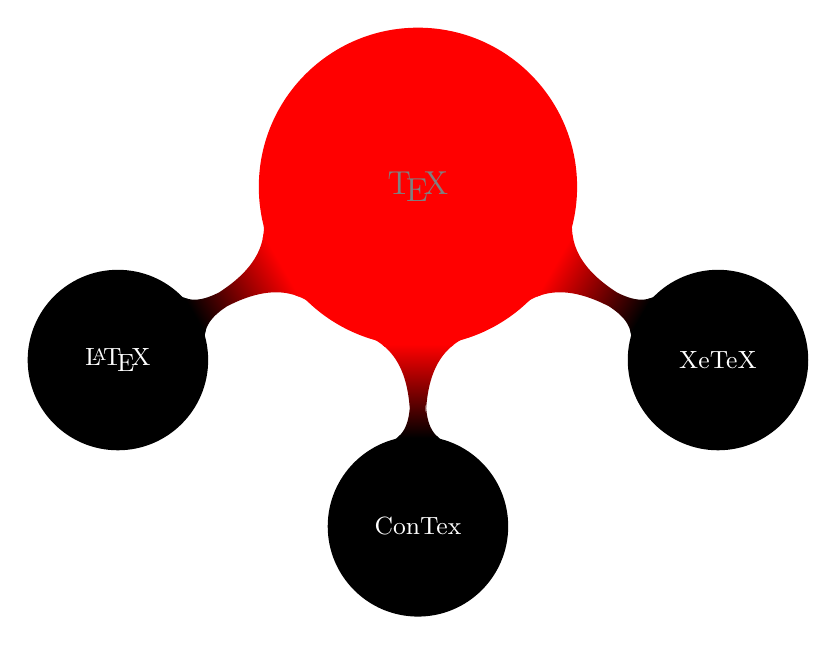
\begin{tikzpicture}[scale=0.88]
        %\tikzset{every child/.append style={level distance=250}}
        \path[mindmap,concept color=red,text=gray,yshift=3cm]
        node[concept] {\TeX}
        [clockwise from=-30]
        child[concept color=black,text=white] { node[concept] {\textcolor{white}{XeTeX}} }
        child[concept color=black,text=white,yshift=0.1cm] { node[concept]{ConTex} }
        child[concept color=black,text=white] { node[concept] {\LaTeX} };
    \end{tikzpicture}%
    % }
\end{frame}

\subsection{Footnote}

\begin{frame}{Footnotes}
    Lorem ipsum dolor sit amet, consetetur sadipscing elitr, sed diam nonumy eirmod tempor invidunt ut labore et dolore magna aliquyam erat, sed diam voluptua. At vero eos et accusam et justo duo dolores et ea rebum. Stet clita kasd gubergren, no sea takimata sanctus est Lorem ipsum dolor sit amet. Lorem \footnote{Lorem ipsum dolor sit amet} ipsum dolor sit amet, consetetur sadipscing elitr, sed diam nonumy eirmod tempor invidunt ut labore et dolore magna aliquyam erat, sed diam voluptua. At vero eos et accusam et justo duo dolores et ea rebum. Stet clita kasd gubergren, no sea takimata sanctus est Lorem ipsum dolor sit amet.
\end{frame}

\subsection{Notes}
\begin{frame}{slide with associated notes slide}
    This slide is for the audience.

    The following programmes are suitable for its presentation:

    \begin{itemize}
        \item Splitshow (Mac OS X)\\url{https://code.google.com/p/splitshow/}
        \item pdf-presenter (Windows)\\url{https://code.google.com/p/pdf-presenter/}
    \end{itemize}
\end{frame}

\note{
    Use this slide for your notes on the presentation.

    The following programmes are suitable for your presentation:

    \begin{itemize}
        \item Splitshow (Mac OS X)\\\url{https://code.google.com/p/splitshow/}
        \item pdf-presenter (Windows)\\\url{https://code.google.com/p/pdf-presenter/}
    \end{itemize}
}

\subsection{Columns}

\begin{frame}{Two columns}
    \begin{multicols}{2}
        Lorem ipsum dolor sit amet, consetetur sadipscing elitr, sed diam nonumy eirmod tempor invidunt ut labore et dolore magna aliquyam erat, sed diam voluptua. At vero eos et accusam et justo duo dolores et ea rebum. Stet clita kasd gubergren, no sea takimata sanctus est Lorem ipsum dolor sit amet.

        \begin{itemize}
            \item one entry
            \item another entry
        \end{itemize}
    \end{multicols}
\end{frame}

\begin{frame}{Column break}
    \begin{multicols}{2}
        Lorem ipsum dolor sit amet, consetetur sadipscing elitr, sed diam nonumy eirmod tempor invidunt ut labore et dolore magna aliquyam erat, sed diam voluptua. At vero eos et accusam et justo duo dolores et ea rebum. Stet clita kasd gubergren, no sea takimata sanctus est Lorem ipsum dolor sit amet.

        \columnbreak
        \begin{itemize}
            \item one entry
            \item another entry
        \end{itemize}
    \end{multicols}
\end{frame}

\section{Future Work and Conclusion}

\begin{frame}{Future Work}
    \begin{itemize}
        \item Do this
        \item Do that
    \end{itemize}
\end{frame}

\begin{frame}{Conclusion}
    In this thesis I explored people's perception of privacy of IoT systems and
    made an application that aims to create more awareness in users about their
    environment and the IoT devices that inhabit it.
\end{frame}

\begin{frame}{Questions and Comments}
    Thank you for your attention. Any questions?
\end{frame}

\begin{frame}{References}
    \begin{thebibliography}{10}
        \beamertemplatebookbibitems
        \bibitem{Oppenheim2009}
        Alan~V.~Oppenheim
        \newblock Discrete-Time Signal Processing
        \newblock Prentice Hall Press, 2009
        \beamertemplatearticlebibitems
        \bibitem{EBU2011}
        European~Broadcasting~Union
        \newblock Specification of the Broadcast Wave Format (BWF)
        \newblock 2011
    \end{thebibliography}
\end{frame}

\end{document}
